\begin{filecontents*}{example.eps}
gsave
newpath
  20 20 moveto
  20 220 lineto
  220 220 lineto
  220 20 lineto
closepath
2 setlinewidth
gsave
  .4 setgray fill
grestore
stroke
grestore
\end{filecontents*}


\RequirePackage{fix-cm}
%
%\documentclass{svjour3}                     % onecolumn (standard format)
\documentclass[smallcondensed]{svjour3}     % onecolumn (ditto)
%\documentclass[smallextended]{svjour3}       % onecolumn (second format)
%\documentclass[twocolumn]{svjour3}          % twocolumn
%
\smartqed  % flush right qed marks, e.g. at end of proof
%
\usepackage{graphicx}
%
% \usepackage{mathptmx}      % use Times fonts if available on your TeX system
%
% insert here the call for the packages your document requires
%\usepackage{latexsym}
% etc.
%
% please place your own definitions here and don't use \def but
% \newcommand{}{}
%
\usepackage{hhline}
\usepackage{natbib}
\usepackage{subfigure}
\usepackage{amssymb}
\usepackage[latin1]{inputenc}
\usepackage[usenames]{color}
%\usepackage{hyperref}

% Insert the name of "your journal" with
 \journalname{Ocean Dynamics}
%
\begin{document}

\title{A simple approach to adjust tidal forcing in fjord models
%\thanks{Grants or other notes
%about the article that should go on the front page should be
%placed here. General acknowledgments should be placed at the end of the article.}
}
%\subtitle{Do you have a subtitle?\\ If so, write it here}

%\titlerunning{Short form of title}        % if too long for running head

\author{K.~Hjelmervik \and N.M.~Kristensen \and A.~Staalstr{\o}m \and L.P.~R{\o}ed
}

%\authorrunning{Short form of author list} % if too long for running head

\institute{K.~Hjelmervik \at
            University College of Southeast Norway\\
            \email{Karina.Hjelmervik@hbv.no}
            \and
            N.M.~Kristensen \at
            Norwegian Meteorological Institute\\
            \and
            A.~Staalstr{\o}m \at
            Norwegian Institute for Water Research\\
            \and
            L.P.~R{\o}ed \at
            Norwegian Meteorological Institute\\
				University of Oslo \\
}

\date{Received: date / Accepted: date}
% The correct dates will be entered by the editor


\maketitle

To model currents in a fjord accurate tidal forcing is of extreme importance. Due to complex topography with narrow and shallow straits, the tides in the innermost parts of a fjord are both shifted in phase and altered in amplitude compared to the tides in the open water outside the fjord.
Commonly, coastal tide information extracted from global or regional models is used on the boundary of the fjord model.
Since tides vary over short distances in shallower waters close to the coast, the global and regional tidal forcings are usually too coarse to achieve sufficiently accurate tides in fjords. We present a straightforward method to remedy this problem by simply adjusting the tides to fit the observed tides at the entrance of the fjord. 
To evaluate the method, we present results from the Oslofjord, Norway. 
%The model we use is a curvilinear version of the Regional Ocean Model System (ROMS) adapted for the Oslofjord. 
A model for the fjord is first run using raw tidal forcing on its open boundary. By comparing modelled and observed time series of water level at a tidal gauge station close to the open boundary of the model, a factor for the amplitude and a shift in phase is computed. The amplitude factor and the phase shift are then applied to produce adjusted tidal forcing at the open boundary. Next we rerun the fjord model using the adjusted tidal forcing. The results from the two runs are then compared to independent observations inside the fjord in terms of amplitude and phases of the various tidal components, the total tidal water level, and the depth integrated tidal currents. The results show improvements in the modelled tides in both the outer, and more importantly, the inner parts of the fjord.

\section{Introduction}

Tides are said to have the longest and most extensive history as a subject of scientific research among all altimetric corrections \cite[]{egbert94,cartwright77,hendershott81}. Already in 1947, the tides was thought to be so well understood that Unna stated that the expressions must not be applied too literally, for that would imply that the tidal wave behave as it ought to do, which is not the case \cite[]{unna47}. Two decades later, Munk and Cartwright apologised for attempting to improve the one geophysical prediction that worked tolerably well already \cite[]{munk66}. Since then numerous scientists have continued to improve the understanding and prediction of tides. 

The tides are especially challenging in coastal waters. Along the Norwegian coast tides are one of the dominant contributor to sea level variations \cite[]{grabbe09}. Numerous fjords with different topography, climatology, and dynamics are affected by tides. For the local communities and industries it is important to improve knowledge of the tides. 

As in many regional models \cite[]{gjevik89}, the tides are often imposed only on the boundary of the fjord models. Close to the coastline, the tides vary over short distances. The TPXO tidal atlases with a horizontal resolution of 1/4$^o$ for the global solution, and 1/30$^o$ for the Atlantic \cite[]{egbert94,egbert02} is too coarse to get the correct phase and amplitude. Here we propose a new method on how to adjust the tidal forcing to improve the forecast of tidal currents in fjord models. 


\section{Area of interest}
Two areas are chosen in this study in order to investigate if the method handles different types of fjords, the Oslo fjord and the Salt- and Skjerstad fjord.

\begin{figure}[!t]
\centering
\includegraphics[width=0.5\textwidth]{fig_Oslofjorden_area}
\caption{The Oslo fjord. The position of the four tide gauges in Oslo, Oscarsborg, Viker, and Helgeroa are marked.}
\label{fig:area1}
\end{figure}

The Oslo fjord is located in the southeastern part of Norway with the main city of Norway in the innermost part of the fjord (Fig.~\ref{fig:area1}). The fjord lies in the most populated area of Norway and it is therefore important to gain knowledge on this fjord. The fjord has an interesting flow pattern due to several river outlets, thresholds, complex topography, storm situations in Skagerak, and atmospheric forcing. 
Even though the mean total tidal elevation is less than 20 cm in the Oslo fjord, the tidal currents are up to 1 m/s due to the narrow straits and thresholds.In connection with storm surge events, a maximum amplitude of 70 cm is observed. The Oslo fjord has an open, southern boundary towards Skagerak which lies in the eastern part of the North Sea. The circulation in the Skagerak is anticlockwise with brackish outflow from the Baltic Sea \cite[]{rodhe96,svendsen96}. 
The inner part of the fjord has two branches. The western branch is almost cut in two by a narrow, shallow, and long sill which is only 11 metes deep, 180 meters wide, and more than 1 km long. This sill causes a relatively strong tidal current, called Svelvikstraumen. The eastern branch also has a sill. Close to Oscarsborg there is a partly man made sill wich consist of an underwater barrier only 1-2 meters deep and extends halfway across the fjord from the western side. Towards the western side there is a natural sill of about 20 meters depth. North of the sill the maximum depth is more than 120 meters in both branches.  This makes the Oslo fjord peculiar among Norwegian fjords in that most of them have the sill at the entrance to the fjord.

\begin{figure}[!t]
\centering
\includegraphics[width=0.8\textwidth]{fig_Saltstraumen_area}
\caption{The Saltstraumen is a strong current in a narrow passage between the Salt fjord and the Skjerstrad fjord. The position of the tide gauge in Bod\o is marked.}
\label{fig:area2}
\end{figure}

The Saltfjord is located in the northern part of Norway (Fig.~\ref{fig:area2}). Saltstraumen is a small straight at the entrance of the Skjerstad fjord and is counted as the world's strongest tidal currents. The difference between the water level before the narrow straight and after the narrow straight can be up to one meter, causing water speeds up to 11 m/s \cite[]{eliassen01}.
The inner part of the fjord system, the Skjerstad fjord, is a deep glacially carved basin separated from the outer part, the Salt fjord, by a sill in the narrow current named Saltstraumen. This fjord system is generally deep, but the depth from the sill to the mouth of Saltfjorden is less than the depth of the inner part, Skjerstadfjorden. The sill in Saltstraumen is about 50 km from the head of the fjord system. The sill depth is 26 m and the depth in the basin inside the sill is more than 500 m: The inner basin and the sill area are connected by a channel which is much deeper and a little wider than Saltstraumen.

The Norwegian Mapping Authority, Hydrographic Service has 23 tide gauges along the Norwegian coast included one at Spitsbergen. Data is available from 1992 up to the current year. Four of the gauges are placed in the Oslo fjord  (Fig.~\ref{fig:area1}) and one close to the open boundary of the Salt fjord (Fig.~\ref{fig:area2}).


\section{Model setup}

The Regional Ocean Model System (ROMS) version 3.6 is applied for both fjords as described in \cite{roed16}. ROMS is a free-surface, terrain-following, primitive equations ocean model widely used by the scientific community for a diverse range of applications \cite[]{shchepetkin05,shchepetkin09,haidvogel08}. 

Both fjord models utilize high-resolution, curvilinear horizontal grids, and terrain-following sigma layers in the vertical using a continuous, double stretching function following \cite{shchepetkin09}. The Oslofjord and Saltfjord models have 42 and 20 vertical layers, respectively. The minimum depth is set to two meters, and for stability reasons some shallow parts of the fjords are omitted. In order to avoid model instability and/or spurious deep currents, the final masked bathymetry is smoothed as described in \cite{roed16}.

%In the horizontal a curvilinear grid with varying grid size is applied (Fig.~\ref{fig:GridSize}). The characteristic grid size, $\Delta s_{i,j}$, is taken as:
%\begin{eqnarray}
%\Delta s_{i,j}^2 \! = \! 
%\left(\!(x_{i+1,j}-x_{i,j})^2\!\! + \!(y_{i+1,j}-y{i,j})^2\! \right)^{\!0.5}\!\!
%\left(\!(x_{i,j+1}-x_{i,j})^2\!\! + \!(y_{i,j+1}-y_{i,j})^2\! \right)^{\!0.5}
%\end{eqnarray}
%Here $i = 1, \cdots, 299$ and $j =1, \cdots, 899$. $x_{i,j}$ and $y_{i,j}$ are the rho-coordinates of element $(i,j)$. (Sp\o rsm\aa l: Er det hensiktsmessig \aa ta med dette?)

%\begin{figure}[!t]
%\centering
%%\includegraphics[width=0.4\textwidth]{Figurer/GridSize}
%\caption{Characteristic grid size in the whole model area.}
%\label{fig:GridSize}
%\end{figure}

The two models have slightly different setup with regards to the external forcing that is applied; the Oslofjord model is run with all realistic forcing, whereas the Saltfjord model is a pure tidal model. 

The necessary atmospheric input (wind, pressure, temperature, humidity, and cloud cover) for the Oslofjord model is extracted from the AROME-MetCoOp model with a grid resolution of 2.5 km \cite[]{muller2015}. Freshwater discharges (rivers) are taken from a database constructed by use of the hydrological model HBV \cite[]{beldring2003}. At the open boundary to the south, the model is nested offline into the NorKyst800 model \cite[]{albretsen11} through daily means of temperature, salinity, currents etc.

For the Saltfjord model, the values at the open boundary to the west is set to a constant value, based on a one year climatology from the NorKyst800 model. No atmospheric forcing or river inputs were applied.

The tidal forcing in terms of tidal elevations and currents are based on the TPXO 7.2 Atlantic database with a horizontal resolution of 1/30$^o$ \cite[]{egbert02} for the Oslofjord model. The global TPXO 7.2 atlas with  horizontal resolution of 1/4$^o$ was applied for the Saltfjord model. 

\section{Method}

The method is straight forward. First the tidal forcing, the Atlantic TPXO with a resolution of 1/30 degree for the Oslofjord model and the TPXO 7.2 with a resolution of 1/4 degree for the Saltfjord model, were imposed at the open boundaries of the fjord models. The simulated time period is 180 days. 

Time series of observed and simulated water level from locations close to the tidal gauge stations close to the open boundaries, were extracted and analysed based on the T\_Tide package described by \cite{pawlowicz02}. For the Oslofjord model, observed and modelled water level are extracted from a location near Viker which lies inside the model domain. For the Saltfjord model, observed and modelled water level are extracted from a location near Bod\o which lies slightly outside the model domain. Ten major tide constitutents of diurnal (K$_1$, P$_1$, and O$_1$), semidiurnal (K$_2$, S$_2$, M$_2$, and N$_2$), and quarter-diurnal (MN$_4$, M$_4$, and MS$_4$) frequencies are retrieved from the observed and modelled time series. 

To better match the observations, the tidal amplitudes and corresponding phase were modified by computing an amplitude factor, $c^{(n)}$, and a phase shift, $\triangle \phi^{(n)}$, for each tidal component $n$ for the water level according to:
\begin{eqnarray}
c^{(n)} &=& \frac{a^{(n)}_{obs}}{a^{(n)}_{sim}} \\
\triangle \phi^{(n)} &=& \phi^{(n)}_{obs} - \phi^{(n)}_{sim}
\end{eqnarray}
$a^{(n)}_{obs}$ and $a{(n)}_{sim}$ are the observed and simulated amplitude respectively. $\phi^{(n)}_{obs}$ and $\phi^{(n)}_{sim}$ are the observed and simulated phase respectively.. 

New amplitudes and phases at the boundary were then calculated using the computed factors and phase shifts on both water level and velocity. The new amplitudes and phases imposed at the open boundaries of new simulations where taken as:
\begin{eqnarray}
a^{(n)}_{i2} &=& a^{(n)}_{i1} c^{(n)} \\
\phi^{(n)}_{i2} &=& \phi^{(n)}_{i1} + \triangle \phi^{(n)}
\end{eqnarray}
$a^{(n)}_{i1}$ and $\phi^{(n)}_{i1}$ are the amplitude and phase originally imposed on grid cell $i$ along the boundary. Modified major and minor amplitude and phase for the tidal current are adjusted in the same way using the amplitude factor and phase shift calculated from the water level. The inclination angles are not adjusted.

The models are then rerun with the adjusted tidal forcing. The results are then analysed as for the first run and  compared with observed tidal water level. 

\section{Discussion and results}

The model is run twice. First with the original tidal forcing. Secondly with the adjusted tidal forcing. The results improved for the Oslo fjord. Table \ref{tab:Viker} shows that the adjustment has the desired effect close to the open boundary. Table \ref{tab:Oscarsborg} shows that the simulated tides are distributed as intended in the inner parts of the fjord. The results also improved for the Salt- and Skjerstad fjord. Table \ref{tab:Bodo} shows that the amplitudes are still too small in the second run, but better than in the first run. The error in phase for M$_2$ was only 0.8 degrees which corresponds to three minutes (Table \ref{tab:Bodo}).

The barotropic tide propagates with a phase speed of $c = \omega/k \approx \sqrt{g h_c}$ where $g$ is the acceleration of gravity and $h_c$ is the characteristic depth. The distance from Viker to Oscarsborg is approximately 75 km and the mean depth is around 200 meters which gives an approximate phase speed of 44 m/s and a phase lag of approximately 28 minuters. According to Table \ref{tab:Viker} and \ref{tab:Oscarsborg} the observed phase lag is 17 degrees for M$_2$ which corresponds to 35 minutes which is only slightly longer than the approximate theoretical phase lag. 

Fields of the amplitude and phase for M$_2$ in the Oslo fjord reveal som interesting phenomenas (Figure \ref{fig:Oslofjord_tidal_fields}). The M$_2$ amplitude decreases gradually from the open boundary in the south.  In the western branch the amplitude decreases as the water pass through the very narrow passage called Svelvikstraumen, while the amplitude increases north of the sill in the eastern branch. The M$_2$ phase decreases in the eastern branch, but increases in the western branch. The observed phase delay is more pronounced in the observations than the model. 

The spatial variation is larger in the Salt fjord. The Saltstraumen is one of the worlds strongest tidal currents. Due to a narrow passage the tidal amplitude is much smaller inside the narrow passage than outside the passage, resulting in strong currents. 
The presence of Saltstraumen as a major impact on the circulation in the Salt fjord. According to \cite{svendsen96} an anticyclonic vortex is formed to the northeast of Saltstraumen, and a cyclonic vortex to the northwest.
% Fra Svendsen et. al 1996
%They are caused by the high velocity water coming out from Saltstraumen on the falling tide, where the velocity reaches a maximum of about 4 m s1: The anti-cyclonic vortex is weaker when the tide is rising, but does not reverse direction. The cyclonic vortex almost vanishes on rising tides. These results are in accordance with the results from Resipientunderskelse (Anon., 1990) where a direct measurement of the velocity field was performed over a time period of 10 days.


\begin{figure}[!t]
\centering
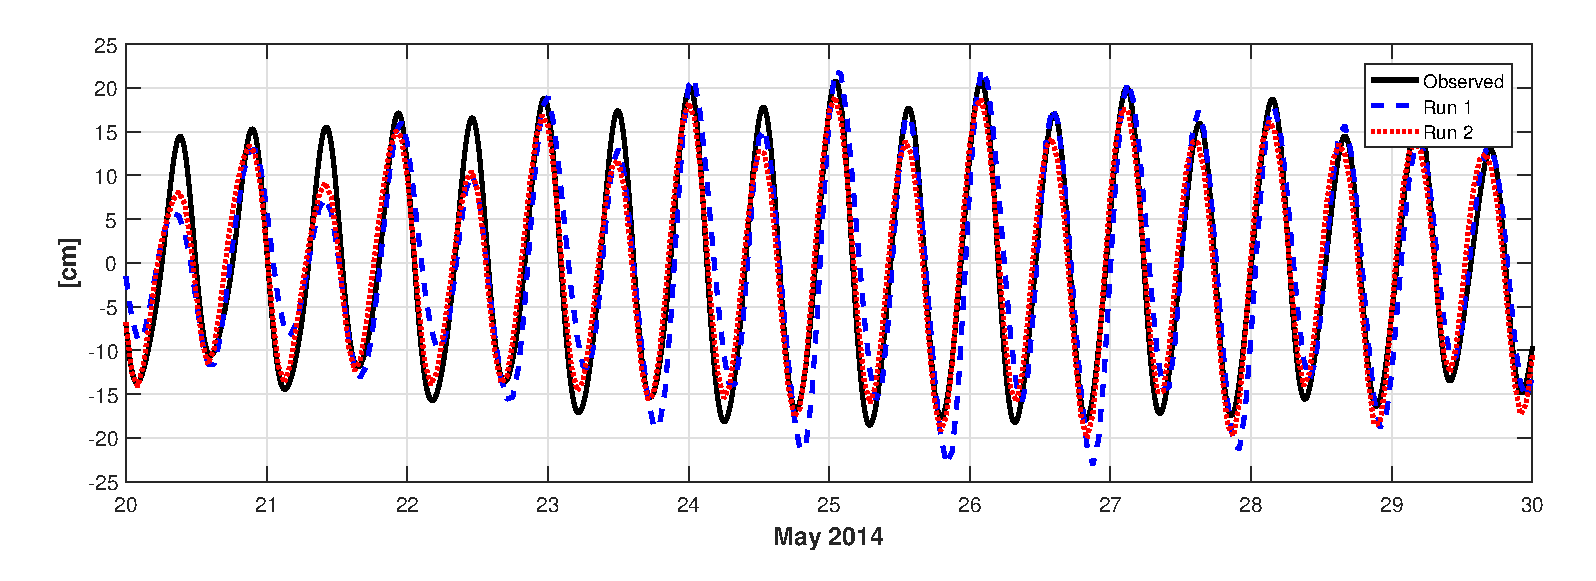
\includegraphics[width=\textwidth]{fig_Viker_timeseries}
\caption{Time series of water level at a position close to Viker}
\label{fig:Viker_timeseries}
\end{figure}



\begin{table}[ht]
%\vspace{-1.5cm}
\caption{Tidal amplitudes [cm] and phases [deg] for the water level at Viker together with adjustment factor $c$ and phase shift $\triangle \phi$ for each component}
\label{tab:Viker}
\centering
\begin{tabular}{crrrrrrrrrr} \hline
       & Period & \multicolumn{2}{c}{Observed} & \multicolumn{2}{c}{Run 1} & \multicolumn{2}{c}{Run 2} & \multicolumn{2}{c}{Adjustment} \\
Comp.  & [h] $\;\;$ & [cm] & [deg] & [cm] & [deg] & [cm] & [deg] & $c\;\;$ & $\triangle \phi$  \\ \hline 
S$_2$  &  12.0000 &   3.0 &  39 &    5.1 &  81 &    3.2 &  67 &    0.588 &   -42.4   \\
M$_2$  &  12.4206 &  11.8 & 105 &    9.7 & 122 &   11.8 & 105 &    1.224 &   -16.8   \\
N$_2$  &  12.6584 &   3.4 &  57 &    5.7 &  81 &    3.1 &  69 &    0.595 &   -24.2   \\
K$_1$  &  23.9345 &   0.7 & 136 &    1.2 & 212 &    0.1 & 198 &    0.554 &   -75.9   \\
P$_1$  &  24.0659 &   0.5 &  66 &    1.2 & 212 &    0.1 & 198 &    0.424 &  -145.5   \\
O$_1$  &  25.8193 &   2.2 & 279 &    3.7 &  19 &    2.9 & 338 &    0.591 &   259.8   \\
MN$_4$ &   6.2692 &   0.4 & 263 &    1.0 & 141 &    0.3 &   7 &    0.368 &   122.2   \\
M$_4$  &   6.2103 &   1.2 & 275 &    0.7 &  25 &    1.1 & 354 &    1.742 &   249.2   \\
MS$_4$ &   6.1033 &   0.3 & 348 &    1.1 & 111 &    0.6 &  80 &    0.272 &   236.7   \\ \hline
\end{tabular}
\end{table}


\begin{table}[ht]
%\vspace{-1.5cm}
\caption{Tidal amplitudes [cm] and phases [deg] for the water level at Oscarsborg}
\label{tab:Oscarsborg}
\centering
\begin{tabular}{crrrrrrrrrr} \hline
      & Period & \multicolumn{2}{c}{Observed} & \multicolumn{2}{c}{Run 1} & \multicolumn{2}{c}{Run 2}  \\
Comp. & [h] $\;\;$ & [cm] & [deg] & [cm] & [deg] & [cm] & [deg]  \\ \hline 
S$_2$  & 12.0000 &  3.6 &  59  &   6.1 &  85  &  3.7 &  69.8  \\
M$_2$  & 12.4206 & 13.7 & 121  &  11.1 & 128  & 13.7 & 111.0  \\
N$_2$  & 12.6584 &  3.9 &  74  &   6.6 &  86  &  3.6 &  75.1  \\
K$_1$  & 23.9345 &  0.9 & 138  &   1.1 & 213  &  0.1 &  44.1  \\
P$_1$  & 24.0659 &  0.7 &  75  &   1.1 & 213  &  0.1 &  44.1  \\
O$_1$  & 25.8193 &  2.4 & 281  &   3.9 &  21  &  3.1 & 340.2  \\
MN$_4$ &  6.2692 &  0.6 & 308  &   2.0 & 163  &  0.5 &  29.1  \\
M$_4$  &  6.2103 &  1.7 & 319  &   1.4 &  44  &  2.0 &  14.5  \\
MS$_4$ &  6.1033 &  0.4 &  32  &   2.2 & 135  &  1.3 & 105.5  \\ \hline 
\end{tabular}
\end{table}




\begin{figure}[!t]
\centering
\includegraphics[trim=1cm 1cm 0cm 0cm,clip=true,width=0.49\textwidth]{fig_Oslofjorden_M2amp.eps}
\includegraphics[trim=1cm 1cm 0cm 0cm,clip=true,width=0.49\textwidth]{fig_Oslofjorden_M2phase.eps}
%\includegraphics[width=0.33\textwidth]{fig_Oslofjorden_M2camp.eps}
\caption{Fields of M$_2$ water level amplitude and phase in the Oslo fjord. The corresponding observed values are indicated by colored cirles at the three permanent gauges in the area.}
\label{fig:Oslofjord_tidal_fields}
\end{figure}


\begin{figure}[!t]
\centering
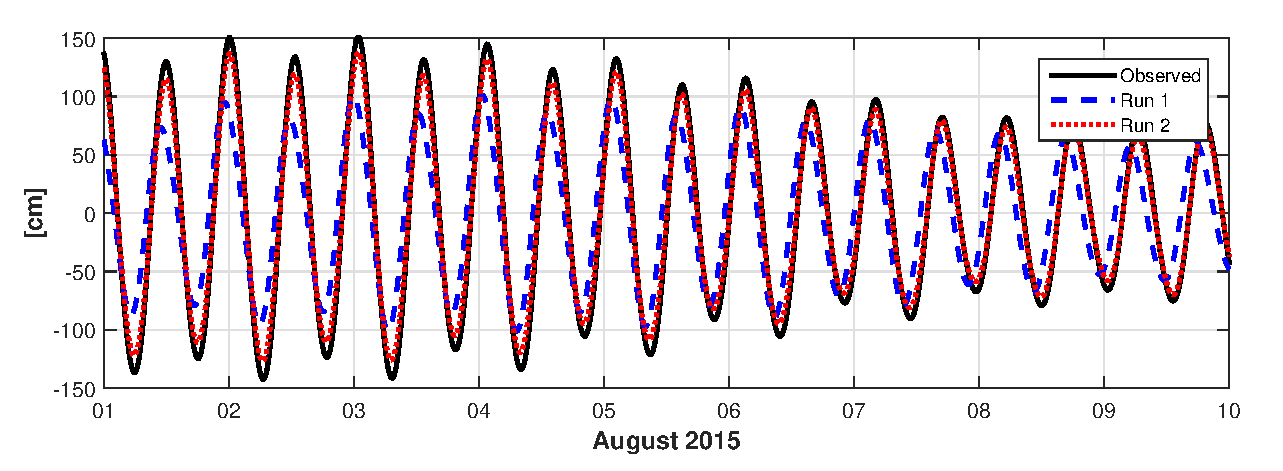
\includegraphics[width=\textwidth]{fig_Saltstraumen_timeseries}
\caption{Time series of water level at a position close to Bod\o}
\label{fig:Saltstraumen_timeseries}
\end{figure}


\begin{figure}[!t]
\centering
\includegraphics[width=\textwidth]{fig_Saltstraumen_M2amp}
\includegraphics[width=\textwidth]{fig_Saltstraumen_M2phase}
\caption{Fields of M$_2$ water level amplitude and phase in the Salt and Skjerstad fjords.}
\label{fig:Saltstraumen_field}
\end{figure}

\begin{table}[ht]
%\vspace{-1.5cm}
\caption{Tidal amplitudes [cm] and phases [deg] for the water level at Bod{\o} together with adjustment factor $c$ and phase shift $\triangle \phi$ for each component}
\label{tab:Bodo}
\centering
\begin{tabular}{crrrrrrrrrr} \hline
      & Period & \multicolumn{2}{c}{Observed} & \multicolumn{2}{c}{Run 1} & \multicolumn{2}{c}{Run 2} & \multicolumn{2}{c}{Adjustment} \\
Comp. & [h] $\;\;$ & [cm] & [deg] & [cm] & [deg] & [cm] & [deg] & $c\;\;$ & $\triangle \phi$  \\ \hline 
S$_2$   & 12.0000  &  30.0 &      8   &  19.1 &     16   &  28.1 &      7    &   1.570  &    -7.2   \\ 
M$_2$   & 12.4206  &  87.3 &    331   &  60.0 &    301   &  78.3 &    330    &   1.454  &    29.8   \\ 
N$_2$   & 12.6584  &  18.5 &    308   &  12.7 &    271   &  16.7 &    309    &   1.461  &    37.2   \\ 
K$_1$   & 23.9345  &  10.8 &    194   &   8.8 &    183   &  10.7 &    194    &   1.225  &    11.5   \\ 
O$_1$   & 25.8193  &   3.8 &     33   &   3.3 &     39   &   3.7 &     33    &   1.154  &    -6.1   \\ 
MN$_4$  &  6.2692  &   1.5 &    229   &   0.4 &    122   &   1.5 &    228    &   3.000  &   106.9   \\ 
M$_4$   &  6.2103  &   2.7 &    268   &   3.3 &    159   &   3.1 &    283    &   0.808  &   109.5   \\ 
MS$_4$  &  6.1033  &   1.3 &      2   &   1.5 &    152   &   1.4 &     30    &   0.861  &  -149.6   \\ \hline
\end{tabular}
\end{table}

\section{Conclusion}

A key factor to modelling currents in any ocean model is accurate tidal forcing. For regional models, this can be taken from a global or regional atlas of tides, like the TPXO or similar. Our experience is that these solutions might not produce adequate accurate results when applied at the mouth of a fjord in a fjord model. This is because the phase speed of the tidal wave can vary close to the coast, and that the coastline and the depth is not properly resolved in the coarse tidal atlases.

We have proposed a new and simple method to adjust tidal forcing. First we run the ocean model with tidal forcing based on the global or regional tidal atlas, for example the global TPXO with a resolution of $1/4$ degree. Secondly, we run harmonic analysis in order to compare the simulated and observed water level for each tidal component. The ratio between observed and simulated amplitude and a phase difference are computed for each tidal component, and then used to adjust the tidal forcing. The same ratio and phase difference is applied on the amplitudes of both water level and current. After this, the model is rerun with adjusted tidal forcing and the results are evaluated against observations.

The method is tested on two different fjord models in two areas in Norway, the Oslofjord and the Salt- and Skjerstadfjord, which includes the famous Saltstraum maelstrom.
 
The results show improvements in the modelled tidal elevations and phases in both models, and suggest that this simple approach is one way of correcting coarse tidal atlases to yield improved results in a fjord model.


\bibliographystyle{apalike}
\bibliography{Bibliography_Tide}

\end{document}
